\documentclass[11pt,a4paper,oneside,fleqn]{article}
%%%%%%%%%%%%%%%%%%%%%%%%%%%%%%%%%%%%%%%%%%%%%%%%%%%%%%%%%%%%%%%%
%  packages
%%%%%%%%%%%%%%%%%%%%%%%%%%%%%%%%%%%%%%%%%%%%%%%%%%%%%%%%%%%%%%%%
\usepackage{amsmath}  % 数学表达式和数学符号
\usepackage{amssymb} % 花体字符
\usepackage{amsthm} % for theorem and proof
\usepackage[UTF8,scheme = plain]{ctex} % 中文支持
\usepackage{lmodern}
\usepackage{iftex}
\usepackage{indentfirst}
\usepackage{enumitem} 
\usepackage{listings} % 显示代码块
\usepackage{float}  % 指定图片位置
\usepackage{subfigure}  %并排子图 共享标题 有子标题
\usepackage{caption}  % 控制图和表格题目/说明文字的样式
\usepackage{graphicx}  % for png image support
\usepackage{algorithm}
\usepackage{algpseudocode}
\usepackage{threeparttable} % for three lines table
\usepackage{multirow}
\usepackage{geometry} % 页面设置
\usepackage{booktabs} % for toprule, midrule and bottomrule
\usepackage{setspace}  % for line space
\usepackage{xcolor}
\usepackage{appendix}
\usepackage[bookmarksnumbered, bookmarksopen = true, colorlinks, linkcolor = blue]{hyperref}  % bookmarksnumbered现实章节序号, bookmarksopen默认打开书签;有色链接, 支持目录跳转;蓝色的目录链接

%% 清除目录项的页号和分隔点
%\usepackage[titles]{tocloft}
%\cftpagenumbersoff{section}
%\cftpagenumbersoff{subsection}
%\cftpagenumbersoff{subsubsection}
%\renewcommand{\cftdot}{}

\geometry{a4paper,left=2cm,right=2cm,top=3cm,bottom=3cm}
%\numberwithin{equation}{section}
\newtheorem{Def}{Definition}
\renewcommand{\algorithmicrequire}{\textbf{Input:}}  % Use Input in the format of Algorithm
\renewcommand{\algorithmicensure}{\textbf{Output:}} % Use Output in the format of Algorithm
\renewcommand{\baselinestretch}{1.5} % Use 1.5 baseline

\captionsetup{labelformat=default,labelsep=period} % Change the colon (:) to the period (.) in caption of tables.
\setlength{\parindent}{2em} % 段落首行缩进2字符

% 定义
\def\degree{${}^{\circ}$}

% 中英文摘要格式
\newcommand{\enabstractname}{Abstract}
\newcommand{\cnabstractname}{ 中文摘要}
\newenvironment{enabstract}{%
  \par\normalsize
  \noindent\mbox{}\hfill{\bfseries \enabstractname}\hfill\mbox{}\par
  \vskip 2.5ex}{\par\vskip 2.5ex}
\newenvironment{cnabstract}{%
  \par\normalsize
  \noindent\mbox{}\hfill{\bfseries \cnabstractname}\hfill\mbox{}\par
  \vskip 2.5ex}{\par\vskip 2.5ex}

% 标题、作者、日期
  \title{\textbf{\huge{这是一个为李四杰准备的中文模板}}}
\author{李四杰, Sijie Li\\
东南大学经济管理学院\\
School of Economics and Management, Southeast University}

%\date{} % 这一行用来去掉默认的日期显示

\newcommand{\supercite}[1]{\textsuperscript{\cite{#1}}}

\renewcommand{\contentsname}{目录} % 目录变为中文

%%%%%%%%%%%%%%%%%%%%%%  论文  %%%%%%%%%%%%%%%
\begin{document}
\maketitle

% 中英文摘要
\begin{cnabstract}
中文摘要
\par\textbf{关键字:}关键字1;关键字2;关键字3
\end{cnabstract}

\begin{enabstract}
English Abstract
\par\textbf{Keywords: }keyword1; keyword2; keyword3
\end{enabstract}

% 正文
% 插入目录
\newpage
\thispagestyle{empty} %no header
\tableofcontents
\thispagestyle{empty} %no header

\newpage
\setcounter{page}{1}
\section{章节1}
\subsection{子章节1}
\subsection{子章节2}

% 插入图片
% 单个图片
\begin{figure}[htbp]
	\centering
	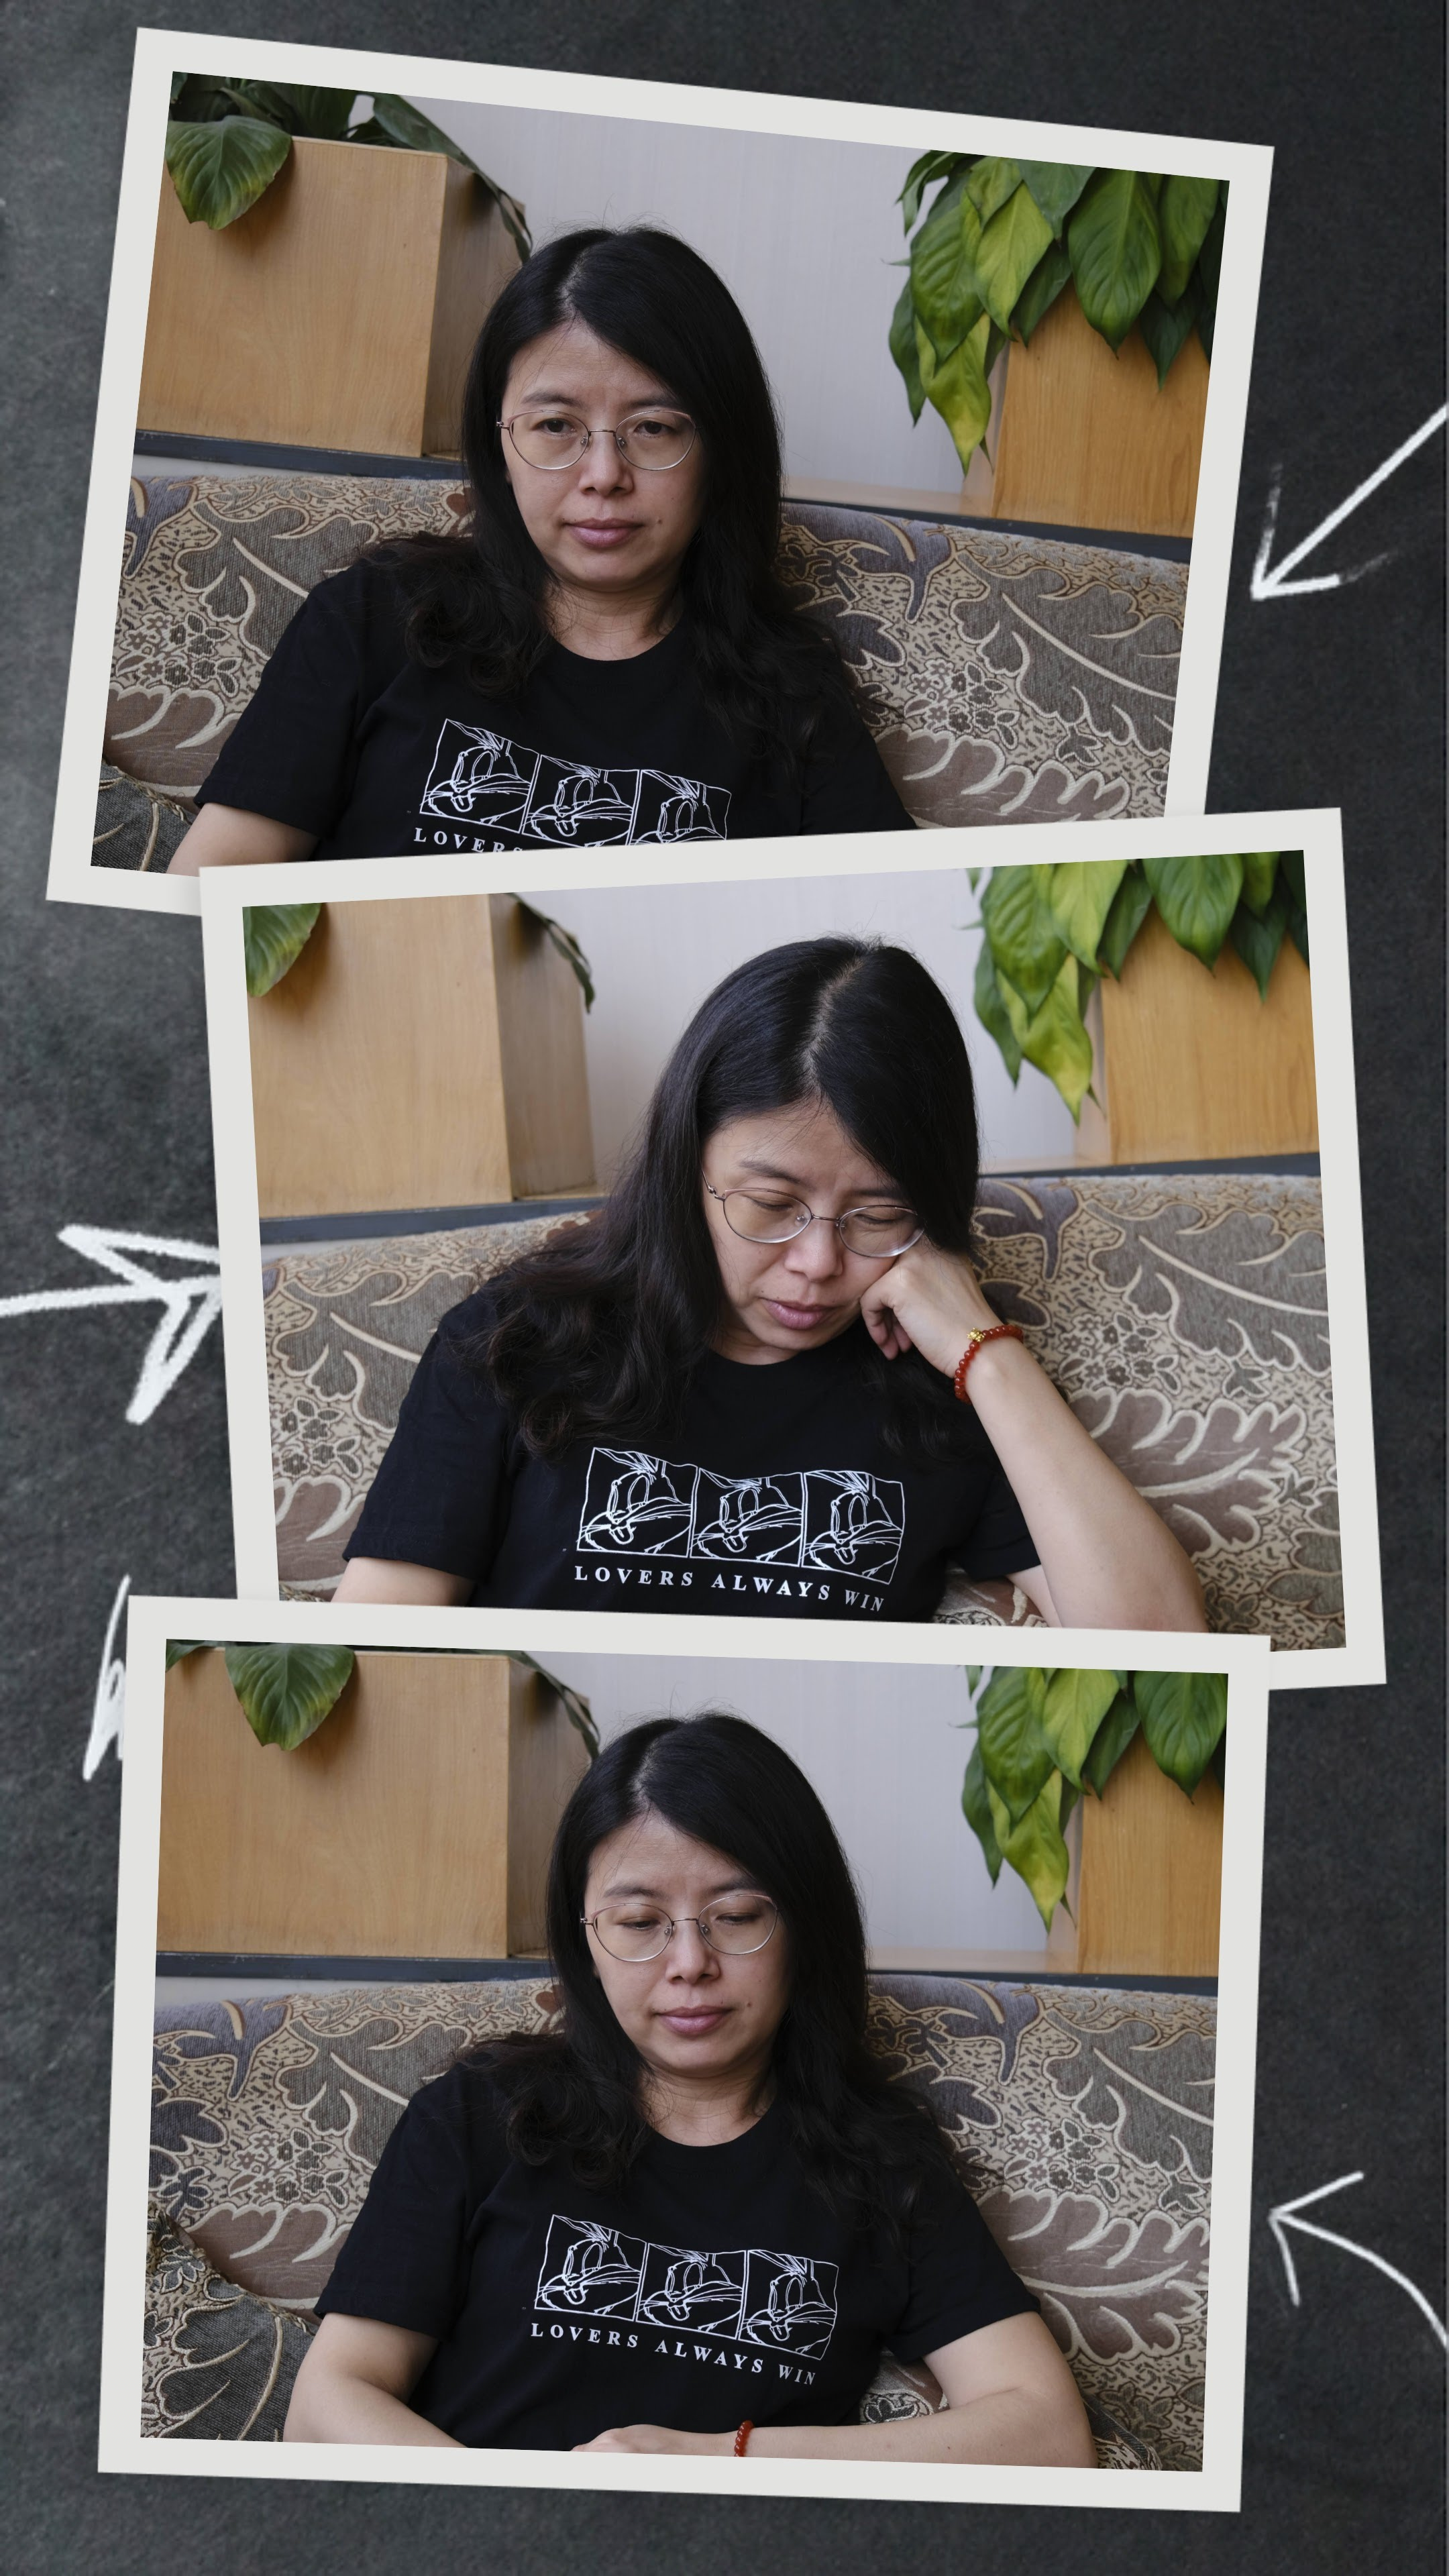
\includegraphics[scale=0.17]{Figs/20210609_171533999_iOS.jpg} %图片路径
	\caption{组合起来的姐姐}
	\label{FIG1-1}
\end{figure}

\begin{figure}[htbp]
  \centering
  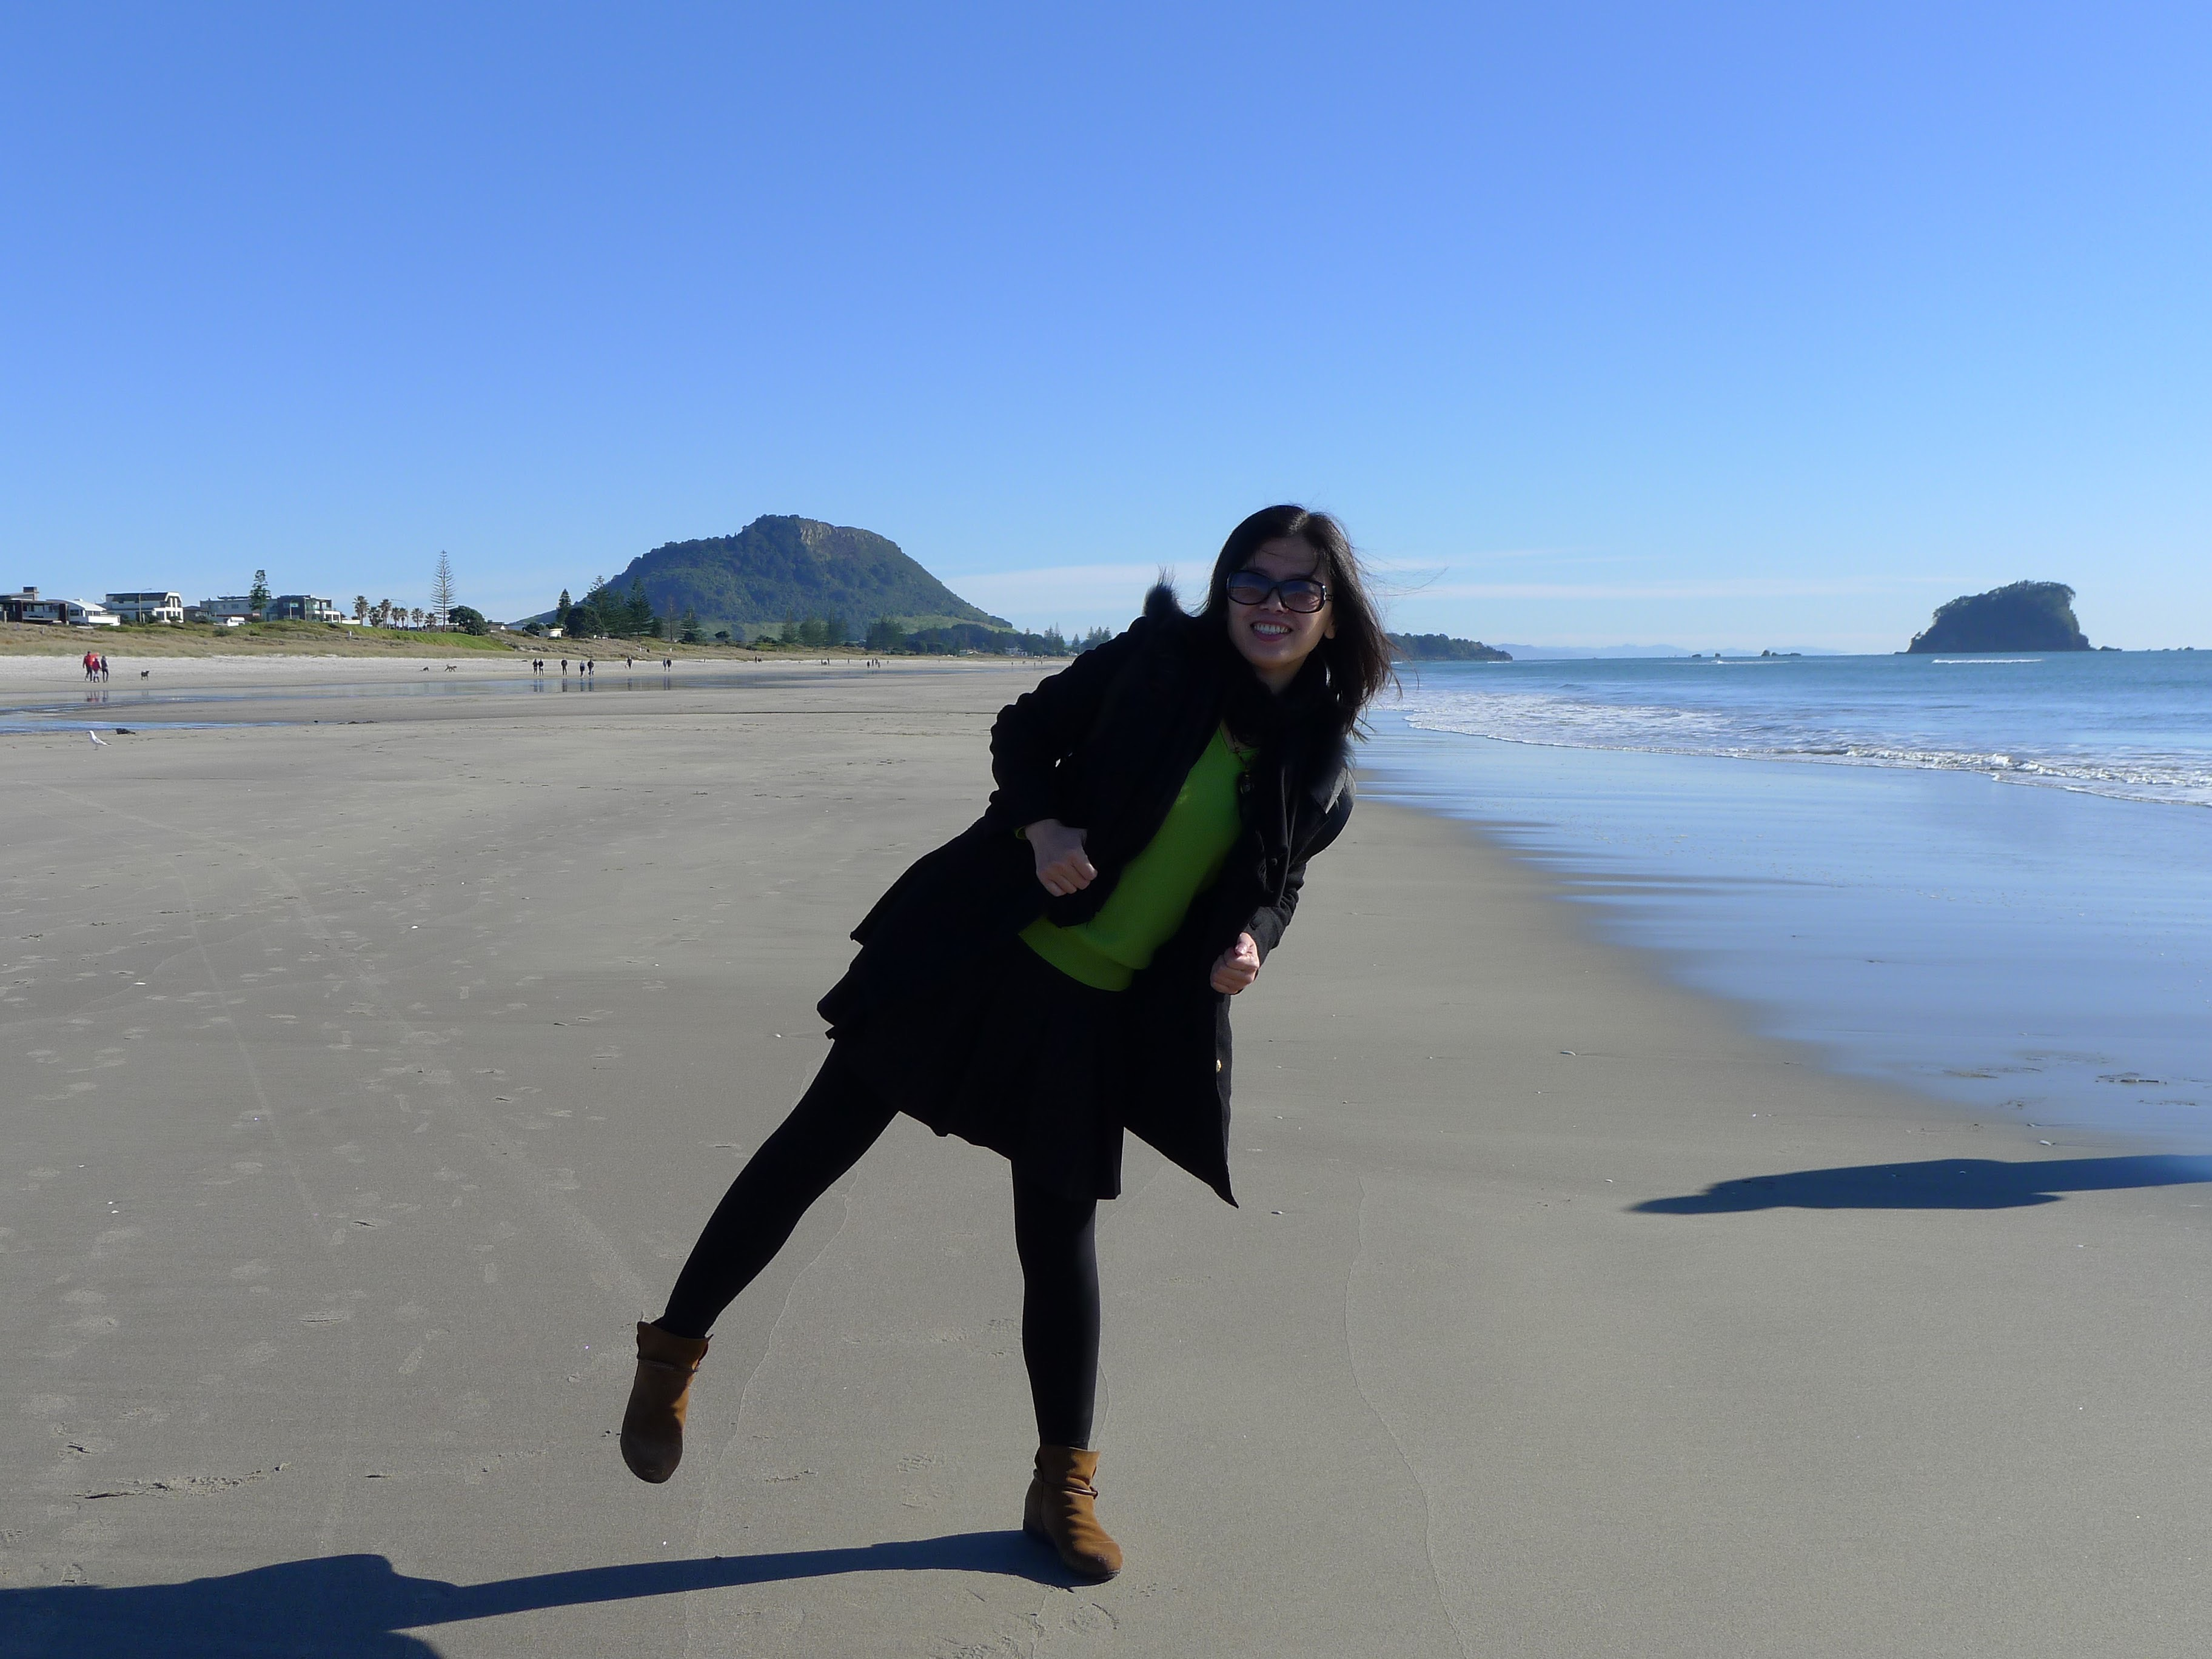
\includegraphics[scale=.13]{Figs/20160703_153846000_iOS.jpg}
  \caption{我亲爱的You姐姐}
  \label{FIG:1-2}
\end{figure}

% 插入表格
\begin{table}[htbp]
\begin{center}
\caption{表格标题}
\begin{tabular}{ccc}% 通过添加 | 来表示是否需要绘制竖线  c|c|c
\toprule  % 在表格最上方绘制横线
	表头1 & 表头2 & 表头3\\
\midrule  %在第一行和第二行之间绘制横线
	数据1 & 数据2 & 数据3\\
  \hline
  数据1 & 数据2 & 数据3\\
\bottomrule % 在表格最下方绘制横线
\end{tabular}
\label{Table1}
\end{center}
\end{table}

% 插入文本框
\begin{center}
\fbox{\shortstack[l]{
文本第一行内容 \\
文本第二行内容 \\
文本最后一行内容}}
\end{center}

% 插入文献
\newpage
\bibliography{reference}	 % reference文件自己编写,BIB	  
\bibliographystyle{IEEEtr} 

% 插入附录
\newpage
\appendix

\section{附录名}
\subsection{子附录名}

Appendix.

\end{document}
